\chapter{Implementierung von Rayden}
\label{cha:Implementierung}

Dieses Kapitel beschreibt die Implementierung von ausgewählten Komponenten des Rayden-Systems. 

\SuperPar
Die Abschnitte \ref{cha:KeywordGrammar} und \ref{cha:StackMachine} zeigen die Grammatik der Sprache Rayden und den Interpretierer für die Ausführung von \enword{Keywords}. Die Abschnitte enthalten Codeausschnitte der Implementierung und Teile der Grammatik.

\SuperPar
Der Abschnitt \ref{cha:Eval} befasst sich mit der Umsetzung von Ausdrücken im Rayden-System. Dazu werden in diesem Abschnitt Auszüge aus der Grammatik der Sprache Rayden und Teile der \enword{RaydenExpressionEvaluator}-Klasse erklärt. Die Klasse \enword{RaydenExpressionEvaluator} ist für die Auswertung der Ausdrücke zuständig. 

\SuperPar
Im Abschnitt \ref{cha:validateKeyword} wird die Validierung von Rayden-Tests gezeigt. Dafür wird das Validierungssystem von xText verwendet. 

\SuperPar
Abgeschlossen wird dieses Kapitel mit dem Abschnitt \ref{cha:implementJSA}, welcher die Integration des Rayden-Systems in die \enword{Java-Scripting-API} zeigt. 

%%------------------------------------------------------------------------------------------------------

\section{Umsetzung der \enword{Keyword}-Grammatik}
\label{cha:KeywordGrammar}

Die Sprache Rayden wurde mit dem xText-Compilerbauwerkzeug umgesetzt. Die Abbildung \ref{fig:keywordGrammar} zeigt einen Auszug aus der Grammatik für die Sprache Rayden. Die Regel \enword{KeywordDecl} beginnt eine Definition eines neuen \enword{Keywords}. Am Beginn der Regel wird die Art des \enword{Keywords} definiert. Eine Beschreibung und Auflistung der Arten ist in Abschnitt \ref{cha:KeywordTypes} enthalten. Danach folgt ein Name für das \enword{Keyword} (\enword{IDEXT}), auf welchen eine geöffnete geschwungene Klammer folgt.

\begin{figure}
\centering
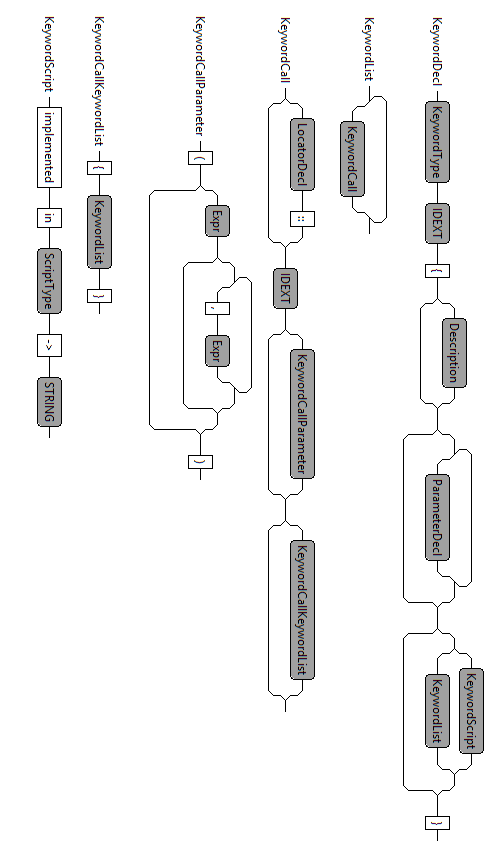
\includegraphics[width=0.9\textwidth]{grammar-keyword-all.png}
\caption{Auszug aus der Grammatik für \enword{Keywords}}
\label{fig:keywordGrammar}
\end{figure}

\SuperPar
Die geschwungenen Klammern definieren den Bereich der \enword{Keyword}-Implementierung. Am Anfang der Implementierung kann eine optionale Beschreibung angeführt werden. Auf diese folgt eine optionale Parameterliste. Ein Parameter wird mit der Regel \enword{ParameterDecl} beschrieben und kann 0 bis \enword{N} Mal wiederholt werden. Eine Parameter-Definition besteht aus dem Schlüsselwort \enword{parameter}, einem Namen, einem optionalen Datentyp und einer Richtung.

\SuperPar
Danach folgt entweder die Bindung an ein Codestück mit der Regel \enword{KeywordScript} oder die \enword{Keyword}-Liste mit der Regel \enword{KeywordList} im Fall eines \enword{Compound Keywords}. Die beiden Angaben sind wiederum optional, um \enword{Keyword}-Rümpfe anlegen zu können. Diese Eigenschaft ist hilfreich, wenn die Testmanagerin oder der Testmanager nur die Struktur festlegen möchte, die Umsetzung des \enword{Keywords} jedoch von anderem Testpersonal vorgenommen wird. 

\SuperPar
Die Regel \enword{KeywordCall} definiert den Aufruf eines \enword{Keywords} in einer \enword{Keyword}-Liste. Die Regel fängt normalerweise mit dem Namen des aufzurufenden \enword{Keywords} an. Danach folgt optional die Parameterliste für den Aufruf eines \enword{Keywords}. Die Regel \enword{KeywordCallParameter} definiert die Parameterliste, welche durch runde Klammern umschlossen ist. Die Parameter können als Liste von \enword{Expr}-Regeln definiert werden und werden durch einen Beistrich separiert. Für die einfachere Verwendung und besserer Lesbarkeit enthält die Regel \enword{KeywordCall} auch noch syntaktischen Zucker. Falls der erste Parameter eines \enword{Keywords} vom Typ \enword{location} ist, kann dieser Parameter vor das \enword{Keyword} geschrieben werden. Somit lässt sich die Implementierung leichter lesen. Der Codeausschnitt \ref{prog:locatorSugar} zeigt dazu die Verwendung dieses syntaktischen Zuckers im Vergleich zur klassischen Verwendung. Am Ende der \enword{KeywordCall}-Regel ist es noch möglich, eine \enword{Keyword}-Liste zu definieren. Diese wird benötigt, falls es sich um ein \enword{Scripted Compound Keyword} oder um ein \enword{Inline Keyword} handelt.

\begin{program}
\begin{JavaCode}
  Type Text (@PetClinic.PetClinicWeb.Login.Username , "max.mustermann")
	@PetClinic.PetClinicWeb.Login.Username :: Type Text ("max.mustermann")
	
	
	Click Left( @PetClinic.PetClinicWeb.Login.Go )
  @PetClinic.PetClinicWeb.Login.Go :: Click Left
\end{JavaCode}
\caption{Syntaktischer Zucker für die Verwendung von \enword{location}-Datentypen}
\label{prog:locatorSugar}
\end{program}


%%------------------------------------------------------------------------------------------------------

\section{Ausführung von \enword{Keywords} mit einer \enword{Stack}-Maschine}
\label{cha:StackMachine}

Im vorigen Abschnitt \ref{cha:KeywordGrammar} wurde die Grammatik eines \enword{Keywords} der Sprache Rayden erklärt. Dieser Abschnitt beschäftigt sich mit der Ausführung von \enword{Keywords}. Damit die \enword{Stack}-Maschine arbeiten kann, benötigt diese den Zugriff auf den abstrakten Syntaxbaum. 

\SuperPar
Das Compilerbauwerkzeug xText stellt für den abstrakten Syntaxbaum ein \enword{Eclipse-ECore}-Modell zur Verfügung. Der generierte Compiler ist so konzipiert, dass dieser die gesamte Quelltextdatei einliest und daraus einen abstrakten Syntaxbaum erzeugt. Dieser abstrakte Syntaxbaum steht für die weitere Verarbeitung als \enword{ECore}-Modell zur Verfügung. Einen Auszug aus dem Modell zeigt die Abbildung \ref{fig:AST}. Diese Abbildung zeigt die Modell-Repräsentation der Grammatik-Regeln von Abbildung \ref{fig:keywordGrammar}. Dieser Ausschnitt aus dem Modell stellt die Basis für die \enword{Stack}-Maschine dar. 

\begin{figure}[h]
\centering
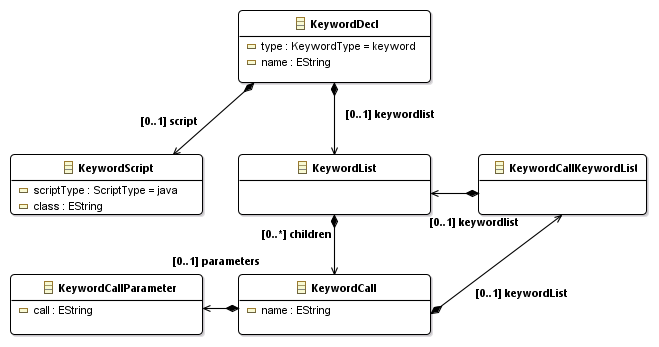
\includegraphics[width=1\textwidth]{keyword-model-diagramm.png}
\caption{Ausschnitt aus dem Grammatik-Modell}
\label{fig:AST}
\end{figure}

\SuperPar
Die \enword{Stack}-Maschine für das Rayden-System ist in der Klasse \enword{RaydenRuntime} implementiert. Der Codeauszug \ref{prog:runtime} zeigt die essentielle Methode \enword{executeKeyword}, welche für die Ausführung von \enword{Keywords} verantwortlich ist. Die Methode wird mit einem \enword{KeywordCall}-Objekt aufgerufen. Dieses Objekt bezeichnet das erste \enword{Keyword}, welches von der \enword{Stack}-Maschine ausgeführt wird. Zuerst werden in der Methode übriggebliebene Elemente vom \enword{Stack} entfernt. Danach werden alle \enword{Reporter-}Objekte über den Start eines neuen Testfalles benachrichtigt. Im nächsten Schritt wird ein neuer Gültigkeitsbereich (\enword{RaydenScriptScope}) angelegt und mit dem \enword{KeywordCall}-Objekt initialisiert. Der Gültigkeitsbereich wird dann auf den leeren \enword{Stack} geladen. 

\SuperPar
Nach der Initialisierung der \enword{Stack}-Maschine wird die Abarbeitung gestartet. Es werden nun solange die \enword{Keywords} am \enword{Stack} abgearbeitet, bis der \enword{Stack} leer oder ein Fehler bei der Ausführung eines \enword{Keywords} aufgetreten ist. Der Gültigkeitsbereich repräsentiert einen Aufruf eines \enword{Keywords} und die dazugehörigen Parameter und Variablen. Der Gültigkeitsbereich speichert zusätzlich die aktuelle Position in der \enword{Keyword}-Liste, falls es sich um ein \enword{Compound Keyword} oder \enword{Scripted Compound Keyword} handelt. Über die Methode \enword{getNextKeyword} kann die \enword{Stack}-Maschine das nächste \enword{Keyword} aus dem aktuellen Gültigkeitsbereich lesen. Liefert die Methode keinen Wert, ist die Ausführung der \enword{Keywords} für diesen Gültigkeitsbereich zu Ende und wird daher vom \enword{Stack} entfernt.

\begin{program}
\lstinputlisting{samplecode/Runtime.java}
\caption{Codeauszug aus der \enword{RaydenRuntime}-Klasse}
\label{prog:runtime}
\end{program}

\SuperPar
Wurde jedoch ein Wert zurückgeliefert, wird mit der Ausführung fortgefahren. Handelt es sich bei dem Wert um ein \enword{KeywordCall}-Objekt, wird die Methode \enword{executeKeywordCall} aufgerufen. Diese Methode löst den Aufruf des \enword{Keywords} über eine \enword{Lookup}-Tabelle auf. Wurde die passende \enword{Keyword}-Implementierung gefunden, wird ein neuer Gültigkeitsbereich angelegt und auf den \enword{Stack} geladen. Wird in der \enword{Lookup}-Tabelle keine passende Implementierung gefunden, wird die Anwendung in einen Fehlerzustand versetzt und die Ausführung abgebrochen. Handelt es sich jedoch um ein \enword{KeywordDecl}-Objekt wird das \enword{Keyword} ausgeführt.  

\SuperPar
Dabei muss die \enword{Stack}-Maschine überprüfen, ob es sich um ein \enword{Scripted Compound Keyword} handelt. Bei einem \enword{Scripted Compound Keyword} muss eine andere Ausführung gewählt werden, da sowohl eine Code-Implementierung, als auch eine \enword{Keyword}-Liste vorhanden sind. Bei allen anderen \enword{Keyword}-Metatypen wird die Methode \enword{executeKeywordDecl} ausgeführt. Diese Methode führt bei einem \enword{Scripted Keyword} das spezifizierte Codestück aus. Bei einem \enword{Compound Keyword} wird die \enword{Keyword}-Liste in den Gültigkeitsbereich geladen.

\SuperPar
Wurden alle Gültigkeitsbereich am \enword{Stack} erfolgreich abgearbeitet, werden am Ende noch alle \enword{Reporter-Objekte} aufgerufen. Danach wird die Ausführung der \enword{Stack}-Maschine beendet.

%%------------------------------------------------------------------------------------------------------
\clearpage

\section{Auswertung von Ausdrücken}
\label{cha:Eval}

Dieser Abschnitt befasst sich mit den Grammatik-Regeln und der Auswertung von Ausdrücken. Die Sprache Rayden unterstützt in einigen Bereichen Ausdrücke. Ein Ausdruck wird in der Grammatik mit der Regel \enword{Expr} beschrieben. Die Abbildung \ref{fig:exprGrammar} zeigt einen Überblick über die Grammatik-Regeln von Ausdrücken. 

\begin{figure}
\centering
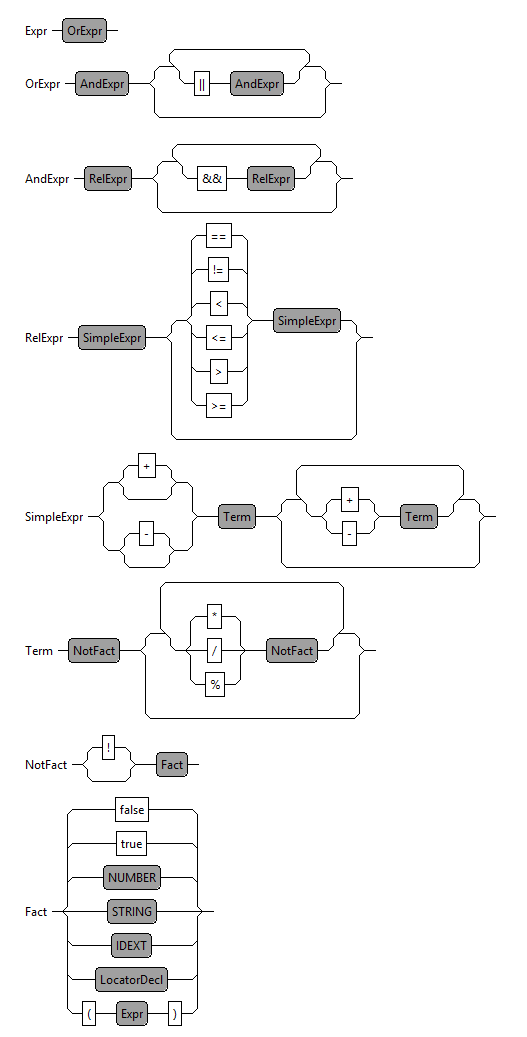
\includegraphics[width=0.9\textwidth]{grammar-expr.png}
\caption{Grammatik-Regeln für Ausdrücke}
\label{fig:exprGrammar}
\end{figure}

\SuperPar
Die Regeln für den Ausdruck sind klassisch aufgebaut. Die Operationen sind nach ihrem Vorrang in den Regeln eingearbeitet. Die am stärksten bindenden Operationen befinden sich dadurch in der Nähe der Blätter des Ausdrucksbaums. Die schwach bindenden Operationen befinden sich in der Nähe des Wurzelknotens. Die Blätter repräsentieren die Werte in einem Ausdruck, welche in der Regel \enword{Fact} definiert werden. Die Werte können entweder Konstanten oder Variablen sein und haben einen definierten Datentypen. Die Regel \enword{Fact} hat jedoch keine spezielle Behandlung für \enword{Enumerations}. Der Grund dafür ist, dass \enword{Enumerations} intern als \enword{Strings} verarbeitet werden. Die Validierung der \enword{Enumerations} wird nur beim Initialisieren von Gültigkeitsbereichen durchgeführt.

\SuperPar
Für die Auswertung von Ausdrücken ist im Rayden-System die Klasse \enword{RaydenExpressionEvaluator} zuständig. Der Codeausschnitt \ref{prog:evaluator} gibt einen Überblick über die Klasse \enword{RaydenExpressionEvaluator}. Ein Objekt dieser Klasse wird mit einem Gültigkeitsbereich initialisiert. Der Gültigkeitsbereich wird benötigt, um Variablen bei der Abarbeitung auswerten zu können. 

\SuperPar
Die Auswertung eines Ausdrucks wird mit der Methode \enword{eval(Expr expression, String resultType)} gestartet. Als Parameter für diese Methode werden ein \enword{Expr}-Objekt und eine Zeichenkette übergeben. Das \enword{Expr}-Objekt ist im \enword{ECore}-Modell das Wurzelobjekt für einen Ausdruck. Mit dem zweiten Parameter \enword{resultType} kann man die Auswertung des Ausdrucks typisieren. Als Wert für den Parameter \enword{resultType} werden die Namen der Datentypen verwendet, welche als Konstanten in dieser Klasse vorhanden sind. Wurde ein Typ definiert, wird am Ende der Auswertung noch überprüft, ob das Ergebnis dem geforderten Typ entspricht. Passt der Wert nicht zum Datentyp, wird eine Ausnahme geworfen. Es gibt auch noch einen Spezialfall bei der Typisierung: Wird ein Ausdruck mit dem Typ \enword{variable} parametrisiert, werden keine Variablen im Ausdruck ausgewertet. Diese Eigenschaft wird benötigt, um Variablennamen an ein \enword{Keyword} übergeben zu können.

\SuperPar
Der Codeausschnitt \ref{prog:evaluator} enthält am Ende die Implementierung der \enword{eval}-Methode für ein Objekt vom Typ \enword{Fact}. Diese Methode zeigt, wie die Werte aus dem \enword{ECore}-Modell nach Java konvertiert werden. Die Methode zeigt auch, wie Variablen mithilfe des Gültigkeitsbereichs ausgewertet werden können.

\begin{program}
\lstinputlisting{samplecode/RaydenExpressionEvaluator.java}
\caption{Codeauszug aus dem \enword{RaydenExpressionEvaluator}}
\label{prog:evaluator}
\end{program}

%%------------------------------------------------------------------------------------------------------
\clearpage
\section{Validierung eines Rayden-Tests}
\label{cha:validateKeyword}

Um die Entwicklung und Wartung von Rayden-Tests zu unterstützen, wurden neben einer syntaktischen Validierung von Tests zusätzliche Validierungen hinzugefügt. Für die Umsetzung der Validierungen wurde eine Schnittstelle des xText-Frameworks verwendet. Nachdem eine Datei erfolgreich durch den xText-Compiler geladen wurde, können zusätzliche Validierungen vorgenommen werden. Der Vorteil bei diesem Vorgehen ist, dass in dieser Phase bereits das gesamte \enword{ECore}-Modell zur Verfügung steht. Die Validierungen können somit für Überprüfungen auf das gesamte Modell zugreifen. In dieser Phase ist auch schon sichergestellt, dass es keine syntaktischen Fehler gibt, da diese Fehler bereits vom Syntaxanalysator gefunden wurden.

\begin{program}
\lstinputlisting{samplecode/Validator.java}
\caption{Codeauszug aus dem \enword{RaydenDSLJavaValidator}}
\label{prog:validator}
\end{program}

\SuperPar
Um Validierungen implementieren zu können, wird von xText eine Klasse generiert, welche mit \enword{JavaValidator} endet. Im Fall von Rayden heißt diese Klasse \enword{RaydenDSLJavaValidator}. In dieser Klasse können nun sprachspezifische Validierungen hinzugefügt werden. Jede Methode in dieser Klasse, welche mit einer \enword{@Check}-Annotation gekennzeichnet ist, wird zur Validierung ausgeführt. 

\SuperPar
Das Codebeispiel \ref{prog:validator} zeigt die Validierung für die Verwendung von \enword{Keywords}. Diese Validierung wird für alle \enword{KeywordCall}-Modellelemente aufgerufen. Ein \enword{KeywordCall} stellt einen Aufruf eines \enword{Keywords} dar. Die Validierung überprüft, ob für jeden Aufruf eines \enword{Keywords} auch eine Implementierung vorhanden ist. Das Traversieren des Modells und Suchen aller Modellelemente entfällt, da diese Aufgabe vom xText-Framework bei jedem neuen Aufruf des Compilers durchgeführt wird.

\SuperPar
Im ersten Schritt überprüft die Validierung aus dem Codebeispiel \ref{prog:validator}, ob es sich um ein \enword{Inline Keyword} handelt: \\

\begin{itemize}

\item Falls das \enword{KeywordCall}-Modellelement ein \enword{Inline Keyword} repräsentiert, kann die Validierung beendet werden, da ein \enword{Inline Keyword} direkt in einem \enword{KeywordCall}-Element implementiert ist. \\

\item Falls es sich nicht um ein \enword{Inline Keyword} handelt, wird im nächsten Schritt in den \enword{Lookup}-Tabellen gesucht, ob eine Implementierung für das \enword{Keyword} vorhanden ist. Wird keine Implementierung gefunden, wird eine Warnung ausgegeben. \\

\end{itemize}

\SuperPar
Das Fehlen einer Implementierung liefert nur eine Warnung. Würde diese Validierung einen Fehler liefern, würde der Compiler aufgrund dieses Fehlers abbrechen und es könnten keine Tests ausgeführt werden, obwohl diese nicht von dem Fehler betroffen wären. Diese Warnung soll vielmehr eine Unterstützung für die Testerinnen und Tester sein, um fehlende \enword{Keyword}-Implementierungen zu finden.

%%------------------------------------------------------------------------------------------------------

\section{Integration von Rayden in die \enword{Java-Scripting-API}}
\label{cha:implementJSA}

Das Rayden-System bietet eine Integration in die \enword{Java-Scripting-API}. Die \enword{Java-Scripting-API} ist eine standardisierte Schnittstelle für das Ausführen von Skriptsprachen in Java. Über diese Schnittstelle kann man direkt in einem Java-Programm ein Skript in einer beliebigen Sprache ausführen. Die einzige Einschränkung dabei ist, dass für die Skriptsprache eine \enword{ScriptEngineFactory} registriert werden muss. Die \enword{Java-Scripting-API} ist vergleichbar mit der \enword{Dynamic Language Runtime} \cite{DLR} in \enword{Microsoft .Net}. Mit der \enword{Dynamic Language Runtime} ist es zum Beispiel in \enword{C\#} möglich, ein Python-Skript \cite{Python} auszuführen.

\begin{figure}
\centering
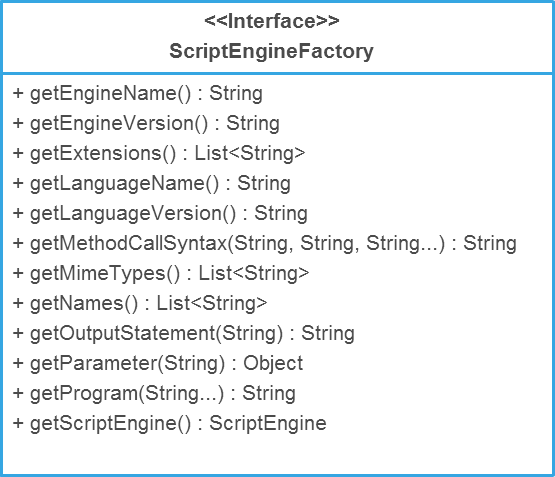
\includegraphics[width=0.7\textwidth]{ScriptEngineFactory.png}
\caption{\enword{ScriptEngineFactory} UML-Klassendiagramm}
\label{fig:scriptEngineFactoryUml}
\end{figure}

\begin{program}
\lstinputlisting{samplecode/ScriptEngine.java}
\caption{Codeauszug aus der \enword{RaydenScriptEngine}}
\label{prog:scriptEngine}
\end{program}

\SuperPar
Für die Integration einer neuen Skriptsprache in die \enword{Java-Scripting-API}, muss man die Schnittstellen \enword{javax.script.ScriptEngineFactory} und \enword{javax.script.ScriptEngine} implementieren. Diese beiden Schnittstellen bilden das Bindeglied zwischen der Java- und der Skriptsprachen-Welt. Die \enword{ScriptEngineFactory}-Schnittstelle liefert Metadaten zu einer Skriptsprache, wie den Namen oder die Versionsnummer. Einen Überblick über die Schnittstelle gibt die Abbildung \ref{fig:scriptEngineFactoryUml}. Die wichtigste Methode der Schnittstelle ist aber \enword{getScriptEngine()}. Diese Methode liefert ein \enword{Script-Engine}-Objekt.

\begin{program}
\lstinputlisting{samplecode/RuntimeLoadFile.java}
\caption{Laden von Rayden-Dateien}
\label{prog:loadFile}
\end{program}

\SuperPar
Über ein \enword{Script-Engine}-Objekt können Skripts ausgeführt werden. Für die Ausführung stehen unterschiedliche Ausprägungen der Methode \enword{eval()} zur Verfügung. Der Skriptcode kann entweder als Zeichenkette oder als \enword{Reader} übergeben werden. Mit einem \enword{Reader} kann man ein Skript direkt aus einer Datei einlesen. Der Codeauszug \ref{prog:scriptEngine} zeigt die Hauptimplementierung der \enword{eval()}-Methode aus der \enword{RaydenScriptEngine}-Klasse. Zu Beginn der Methode wird die Rayden-\enword{Runtime} instanziiert und initialisiert. Die \enword{Runtime} wird benötigt, um einen Rayden-Test ausführen zu können. Im nächsten Schritt wird überprüft, ob ein spezieller \enword{Reporter} verwendet werden soll. Standardmäßig wird die \enword{RaydenXMLReporter}-Implementierung verwendet, welche die gesamten Ausgaben einer Test-Ausführung in einer XML-Datei protokolliert. 

\SuperPar
Damit man in einem Rayden-Test eine Bibliothek verwenden kann, ist es für die Rayden-\enword{Runtime} entscheidend, dass spezifiziert ist, wo die Bibliotheken gefunden werden. Dafür wird ein Arbeitsbereich (\enword{Working Folder}) definiert, in welchem Bibliotheken und andere externe Ressourcen gesucht werden. Der Arbeitsbereich ist standardmäßig das Ausführungsverzeichnis der Java-Anwendung. Der Wert kann aber über einen Kontextparameter verändert werden. Kontextparameter werden verwendet, um Parameter an die \enword{Script Engine} übergeben zu können. 

\SuperPar
Nachdem alle Einstellungen für die Rayden-\enword{Runtime} vorgenommen wurden, wird das Skript mit allen Abhängigkeiten geladen. Dazu wird das Skript mit der Methode \enword{loadRaydenFile()} geladen. Die Implementierung der Methode zeigt der Codeauszug \ref{prog:loadFile}. Wie im Codeauszug dargestellt, gibt es zwei Methoden für das Laden von Rayden-Dateien. Eine Rayden-Datei wird durch die Dateiendung \enword{rlg} identifiziert. Die erste Methode \enword{loadRaydenFile()} ist für das Laden der primären Rayden-Datei zuständig. Mit der zweiten Methode \enword{loadLibraryFile()} werden Bibliotheken geladen. Der Hauptgrund für die zwei unterschiedlichen Methoden ist der, dass zwei \enword{Lookup}-Tabellen für \enword{Keywords} vorhanden sind. Es werden alle \enword{Keywords} aus der primären Rayden-Datei in eine spezielle \enword{Lookup}-Tabelle geladen, sodass nur \enword{Keywords} aus dieser Datei ausgeführt werden können.

\SuperPar
Zum Laden der Rayden-Datei wird der generierte xText-\enword{Parser} verwendet. Im nächsten Schritt wird das Ergebnis des \enword{Parsers} abgefragt und auf Fehler überprüft. Bei einem Fehler wird die Ausführung sofort beendet. Konnte die Datei ohne Fehler geladen werden, liefert der \enword{Parser} eine Instanz des \enword{ECore}-Modells. Das Modell wird durchlaufen und alle \enword{Keyword}-Namen, die gefunden werden, in der \enword{Lookup}-Tabelle gespeichert. Im letzten Schritt werden noch alle Bibliotheken geladen. Das Laden einer Bibliothek funktioniert identisch wie das Laden der primären Rayden-Datei, nur werden in diesem Fall die \enword{Keywords} in eine andere \enword{Lookup}-Tabelle gespeichert. 

\SuperPar
Nachdem das Skript und alle externen Ressourcen erfolgreich geladen wurden, können die Rayden-Tests ausgeführt werden. Dazu stellt die Rayden-\enword{Runtime} die Methode \enword{executeAllTestSuites()} zur Verfügung. Die Methode sucht in der primären \enword{Lookup}-Tabelle nach \enword{Keywords} mit einem Testtyp. 

\SuperPar
Die Sprache Rayden unterstützt folgende Testtypen:

\begin{itemize}
\item Test-Suite (\enword{TestSuite}),
\item Testfall (\enword{TestCase}),
\item Komponententest (\enword{UnitTest}),
\item Integrationstest (\enword{IntegrationTest}),
\item Schnittstellentest (\enword{APITest}),
\item automatisierter Abnahmetest (\enword{AUTest}) und
\item manueller Abnahmetest (\enword{MAUTest}).
\end{itemize}

\SuperPar
Alle gefunden Tests werden im nächsten Schritt sequenziell ausgeführt. Als Resultat der Skriptausführung wird das kumulierte Ergebnis der Tests geliefert. Das Ergebnis kann dann entweder in der Java-Anwendung, welche die Tests gestartet hat, oder nachträglich über die XML-Datei ausgewertet werden.

\SuperPar
In diesem Kapitel wurde für einige essentielle Komponenten des Rayden-Systems gezeigt wie diese umgesetzt wurden. Im nächsten Kapitel wird erläutert, wie man Tests mit dem Rayden-System schreiben und ausführen kann. Dazu werden unterschiedliche Testmethoden verwendet, um die Stärken von Rayden zu demonstrieren.
